% Options for packages loaded elsewhere
\PassOptionsToPackage{unicode}{hyperref}
\PassOptionsToPackage{hyphens}{url}
\documentclass[
  ignorenonframetext,
]{beamer}
\newif\ifbibliography
\usepackage{pgfpages}
\setbeamertemplate{caption}[numbered]
\setbeamertemplate{caption label separator}{: }
\setbeamercolor{caption name}{fg=normal text.fg}
\beamertemplatenavigationsymbolsempty
% remove section numbering
\setbeamertemplate{part page}{
  \centering
  \begin{beamercolorbox}[sep=16pt,center]{part title}
    \usebeamerfont{part title}\insertpart\par
  \end{beamercolorbox}
}
\setbeamertemplate{section page}{
  \centering
  \begin{beamercolorbox}[sep=12pt,center]{section title}
    \usebeamerfont{section title}\insertsection\par
  \end{beamercolorbox}
}
\setbeamertemplate{subsection page}{
  \centering
  \begin{beamercolorbox}[sep=8pt,center]{subsection title}
    \usebeamerfont{subsection title}\insertsubsection\par
  \end{beamercolorbox}
}
% Prevent slide breaks in the middle of a paragraph
\widowpenalties 1 10000
\raggedbottom
\AtBeginPart{
  \frame{\partpage}
}
\AtBeginSection{
  \ifbibliography
  \else
    \frame{\sectionpage}
  \fi
}
\AtBeginSubsection{
  \frame{\subsectionpage}
}
\usepackage{iftex}
\ifPDFTeX
  \usepackage[T1]{fontenc}
  \usepackage[utf8]{inputenc}
  \usepackage{textcomp} % provide euro and other symbols
\else % if luatex or xetex
  \usepackage{unicode-math} % this also loads fontspec
  \defaultfontfeatures{Scale=MatchLowercase}
  \defaultfontfeatures[\rmfamily]{Ligatures=TeX,Scale=1}
\fi
\usepackage{lmodern}
\ifPDFTeX\else
  % xetex/luatex font selection
\fi
% Use upquote if available, for straight quotes in verbatim environments
\IfFileExists{upquote.sty}{\usepackage{upquote}}{}
\IfFileExists{microtype.sty}{% use microtype if available
  \usepackage[]{microtype}
  \UseMicrotypeSet[protrusion]{basicmath} % disable protrusion for tt fonts
}{}
\makeatletter
\@ifundefined{KOMAClassName}{% if non-KOMA class
  \IfFileExists{parskip.sty}{%
    \usepackage{parskip}
  }{% else
    \setlength{\parindent}{0pt}
    \setlength{\parskip}{6pt plus 2pt minus 1pt}}
}{% if KOMA class
  \KOMAoptions{parskip=half}}
\makeatother
\setlength{\emergencystretch}{3em} % prevent overfull lines
\providecommand{\tightlist}{%
  \setlength{\itemsep}{0pt}\setlength{\parskip}{0pt}}
\usepackage{bookmark}
\IfFileExists{xurl.sty}{\usepackage{xurl}}{} % add URL line breaks if available
\urlstyle{same}
\hypersetup{
  hidelinks,
  pdfcreator={LaTeX via pandoc}}

\author{\texorpdfstring{}{}}
\date{}

\begin{document}

\begin{frame}[fragile]{Supplement: Validation and outputs}
\protect\phantomsection\label{supplement-validation-and-outputs}
\begin{figure}[!ht]
\centering
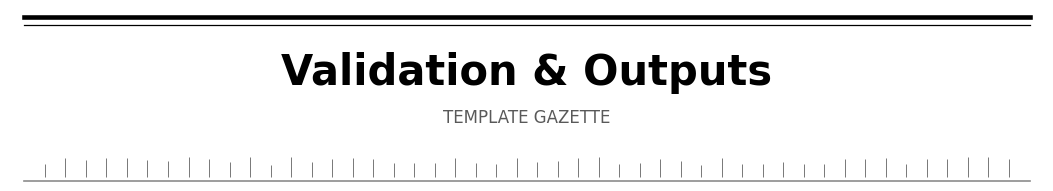
\includegraphics[width=\linewidth]{../figures/section_banner_S03_validation_and_outputs.png}
\caption{Validation supplement banner (B\&W).}
\label{fig:banner_S03_validation_and_outputs}
\end{figure}
\begin{figure}[!ht]
\centering
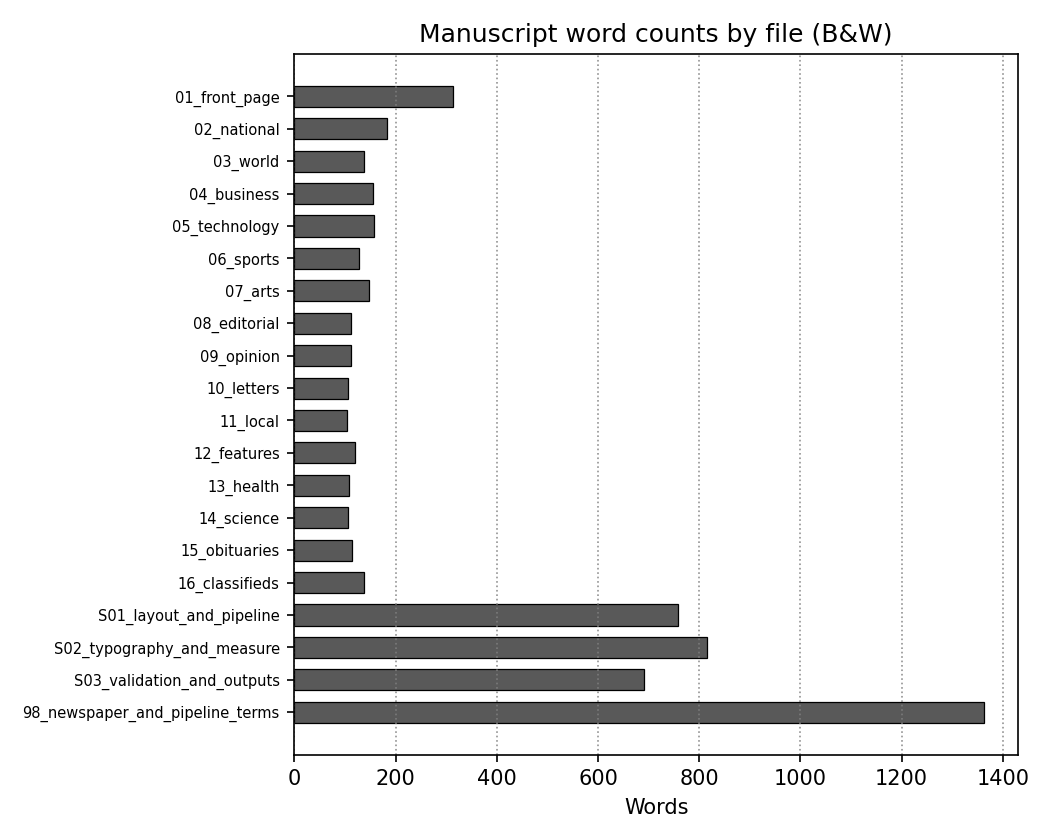
\includegraphics[width=0.92\linewidth]{../figures/wordcount_bars_bw.png}
\caption{Black-and-white horizontal bar chart of word counts per manuscript slice, generated from \texttt{manuscript\_stats.json} by \texttt{visualization\_wordcount\_bw.py} (runs after \texttt{report\_manuscript\_stats.py} in analysis). Bars use grayscale fills only.}
\label{fig:wordcount_bw}
\end{figure}
\begin{multicols}{3}

Figure\textasciitilde{}\ref{fig:wordcount_bw} summarizes edition word
counts for quick sanity checks alongside validators below.

\textbf{Markdown validation.} Run
\texttt{python3\ -m\ infrastructure.validation.cli\ markdown\ projects/traditional\_newspaper/manuscript/}
before large merges. The CLI checks reference integrity, image paths,
and other structural rules configurable per project. Failures should
block PDF generation in CI the same way failing tests do.

\textbf{PDF validation.} After render,
\texttt{python3\ -m\ infrastructure.validation.cli\ pdf\ output/traditional\_newspaper/pdf/}
scans for unresolved citations (\texttt{{[}?{]}}), reference tokens
(\texttt{??}), and common LaTeX warnings surfaced in text extraction.
Treat warnings as debt even when builds succeed.

\textbf{Combined artifact paths.} Combined markdown often lands at
\texttt{output/traditional\_newspaper/pdf/\_combined\_manuscript.md}
during debugging; the compiled PDF is
\texttt{traditional\_newspaper\_combined.pdf} (exact names follow
renderer conventions). Individual section PDFs help bisect errors when
one slice breaks LaTeX.

\textbf{Web output.} \texttt{WebRenderer} produces HTML under
\texttt{output/traditional\_newspaper/web/}. Figures embedded via raw
LaTeX become \texttt{\textless{}figure\textgreater{}} elements when Lua
filters recognize \texttt{\textbackslash{}begin\{figure\}} blocks.
Verify captions render after changing caption text.

\textbf{Slides.} Beamer slides per stem land in
\texttt{output/traditional\_newspaper/slides/}. Slide builds can fail
independently of the combined PDF if a single section includes
incompatible raw TeX---keep slides in CI if your team relies on them.

\textbf{Data outputs.} \texttt{manuscript\_stats.json} tracks word
counts. \texttt{visualization\_wordcount\_bw.py} reads that JSON and
writes \texttt{output/figures/wordcount\_bars\_bw.png} (monochrome bar
chart, Figure\textasciitilde{}\ref{fig:wordcount_bw}).

\textbf{Integrity and checksums.} Optional integrity modules hash
outputs for provenance. Steganography tooling (\texttt{secure\_run.sh})
post-processes PDFs without mutating originals; security-focused teams
may enable it.

\textbf{Failure triage order.} When a build breaks, read the LaTeX log
tail, identify the first undefined control sequence or missing file, fix
that, and rebuild. Pandoc errors precede LaTeX errors chronologically in
logs---start at the earliest failure.

\textbf{Environment reproducibility.} Document \texttt{uv} version,
Python version, and TeX distribution in your lab handbook. Container
images in \texttt{infrastructure/docker/} help teammates match
environments without sharing laptops.

\textbf{Cross-project lessons.} Other projects in the monorepo use the
same validation entry points; fixes to shared infrastructure benefit
everyone. File issues upstream when validators misfire on legitimate
markdown patterns.

\textbf{Longer read: operational playbooks.} Treat validation logs like
server logs: keep the last N successful artifacts, timestamp them, and
attach commit SHAs. When a professor or reviewer asks ``which PDF did
you mean?'', the answer should be a git tag plus a CI run ID, not ``the
one on my desktop.'' Copy stages that mirror \texttt{projects/*/output/}
into \texttt{output/*/} exist precisely so deliverable paths stabilize
for that conversation.

\textbf{Bisection tactics.} If combined PDF fails but individual slices
succeed, binary-search which stem introduces the fault by temporarily
moving half the markdown files aside---careful not to break
\texttt{validate\_inventory}---or by compiling partial combined
markdown. Another approach: inspect \texttt{\_combined\_manuscript.tex}
around the error line LaTeX reports.

\textbf{Performance.} Full XeLaTeX passes dominate pipeline time for
large manuscripts. Caching unchanged slices is tempting but risks stale
cross-references; prefer incremental development on single sections via
\texttt{03\_render\_pdf.py} flags when available, then full combined
builds before release.

\textbf{Artifact hygiene.} \texttt{output/} directories are disposable
per project policy, yet humans treat them as precious.
\texttt{.gitignore} keeps binaries out of version control; document
regeneration commands in README so newcomers are not afraid to delete
stale PDFs.

\textbf{Security scanning.} PDFs can embed JavaScript or launch actions;
validators may flag anomalies. Trusted toolchains reduce surprise. Do
not paste untrusted LaTeX from the internet into \texttt{preamble.md}
without review.

\textbf{Accessibility retesting.} When figure captions change, rerun
HTML export and spot-check screen-reader order: does the caption
immediately follow the image in the DOM? Lua filter ordering can affect
results.

\textbf{Localization.} Validation messages from CLIs are English today;
wrapping them for i18n would help global teams. Manuscript content can
be non-English if fonts and hyphenation languages align---validators
should remain locale-agnostic.

\textbf{Contract tests.} \texttt{validate\_inventory} is a contract:
filenames implied by \texttt{sections.py} must exist. Adding optional
supplements requires updating that tuple---treat it like an API semver
bump for downstream stats scripts.

\textbf{Hand-off checklist.} Before declaring a release: all tests
green, markdown validation clean, PDF validation clean, figures
regenerated, \texttt{manuscript\_stats.json} refreshed, and a human
skimmed captions for typos. Automation covers everything except the last
step---for now.

\end{multicols}
\end{frame}

\end{document}
